\documentclass{article}

\usepackage[final]{nips_2016}

\usepackage[utf8]{inputenc} % allow utf-8 input
\usepackage[T1]{fontenc}    % use 8-bit T1 fonts
\usepackage{hyperref}       % hyperlinks
\usepackage{url}            % simple URL typesetting
\usepackage{booktabs}       % professional-quality tables
\usepackage{amsfonts}       % blackboard math symbols
\usepackage{nicefrac}       % compact symbols for 1/2, etc.
\usepackage{microtype}      % microtypography
\usepackage{amsmath}
\usepackage{color,graphicx}

\title{Deep Learning --- Assignment 4}

\author{Anirudhan J.~Rajagopalan \\
  Department of Computer Science\\
  New York University\\
  New York, NY.\\
  \texttt{ajr619@nyu.edu} \\
}

\begin{document}

\maketitle

\section{nnGraph}
\subsection{1. Warmup}
The code for nngraph\_warmup.lua can be found at \url{https://git.io/vwQco}

\subsubsection{2. Grucell diagram}
The gru cell was drawn using the following steps.
\begin{enumerate}
  \item Code the cell in torch similar to the code in main.lua
  \item Plot the code using graph.dot function passing the filename argument
  \item Open the .svg file in browser and remove the unwanted nodes.
\end{enumerate}

The cell diagram generated is included in~\ref{fig:gru_cell}.

\begin{figure}[ht!]
  \centering
  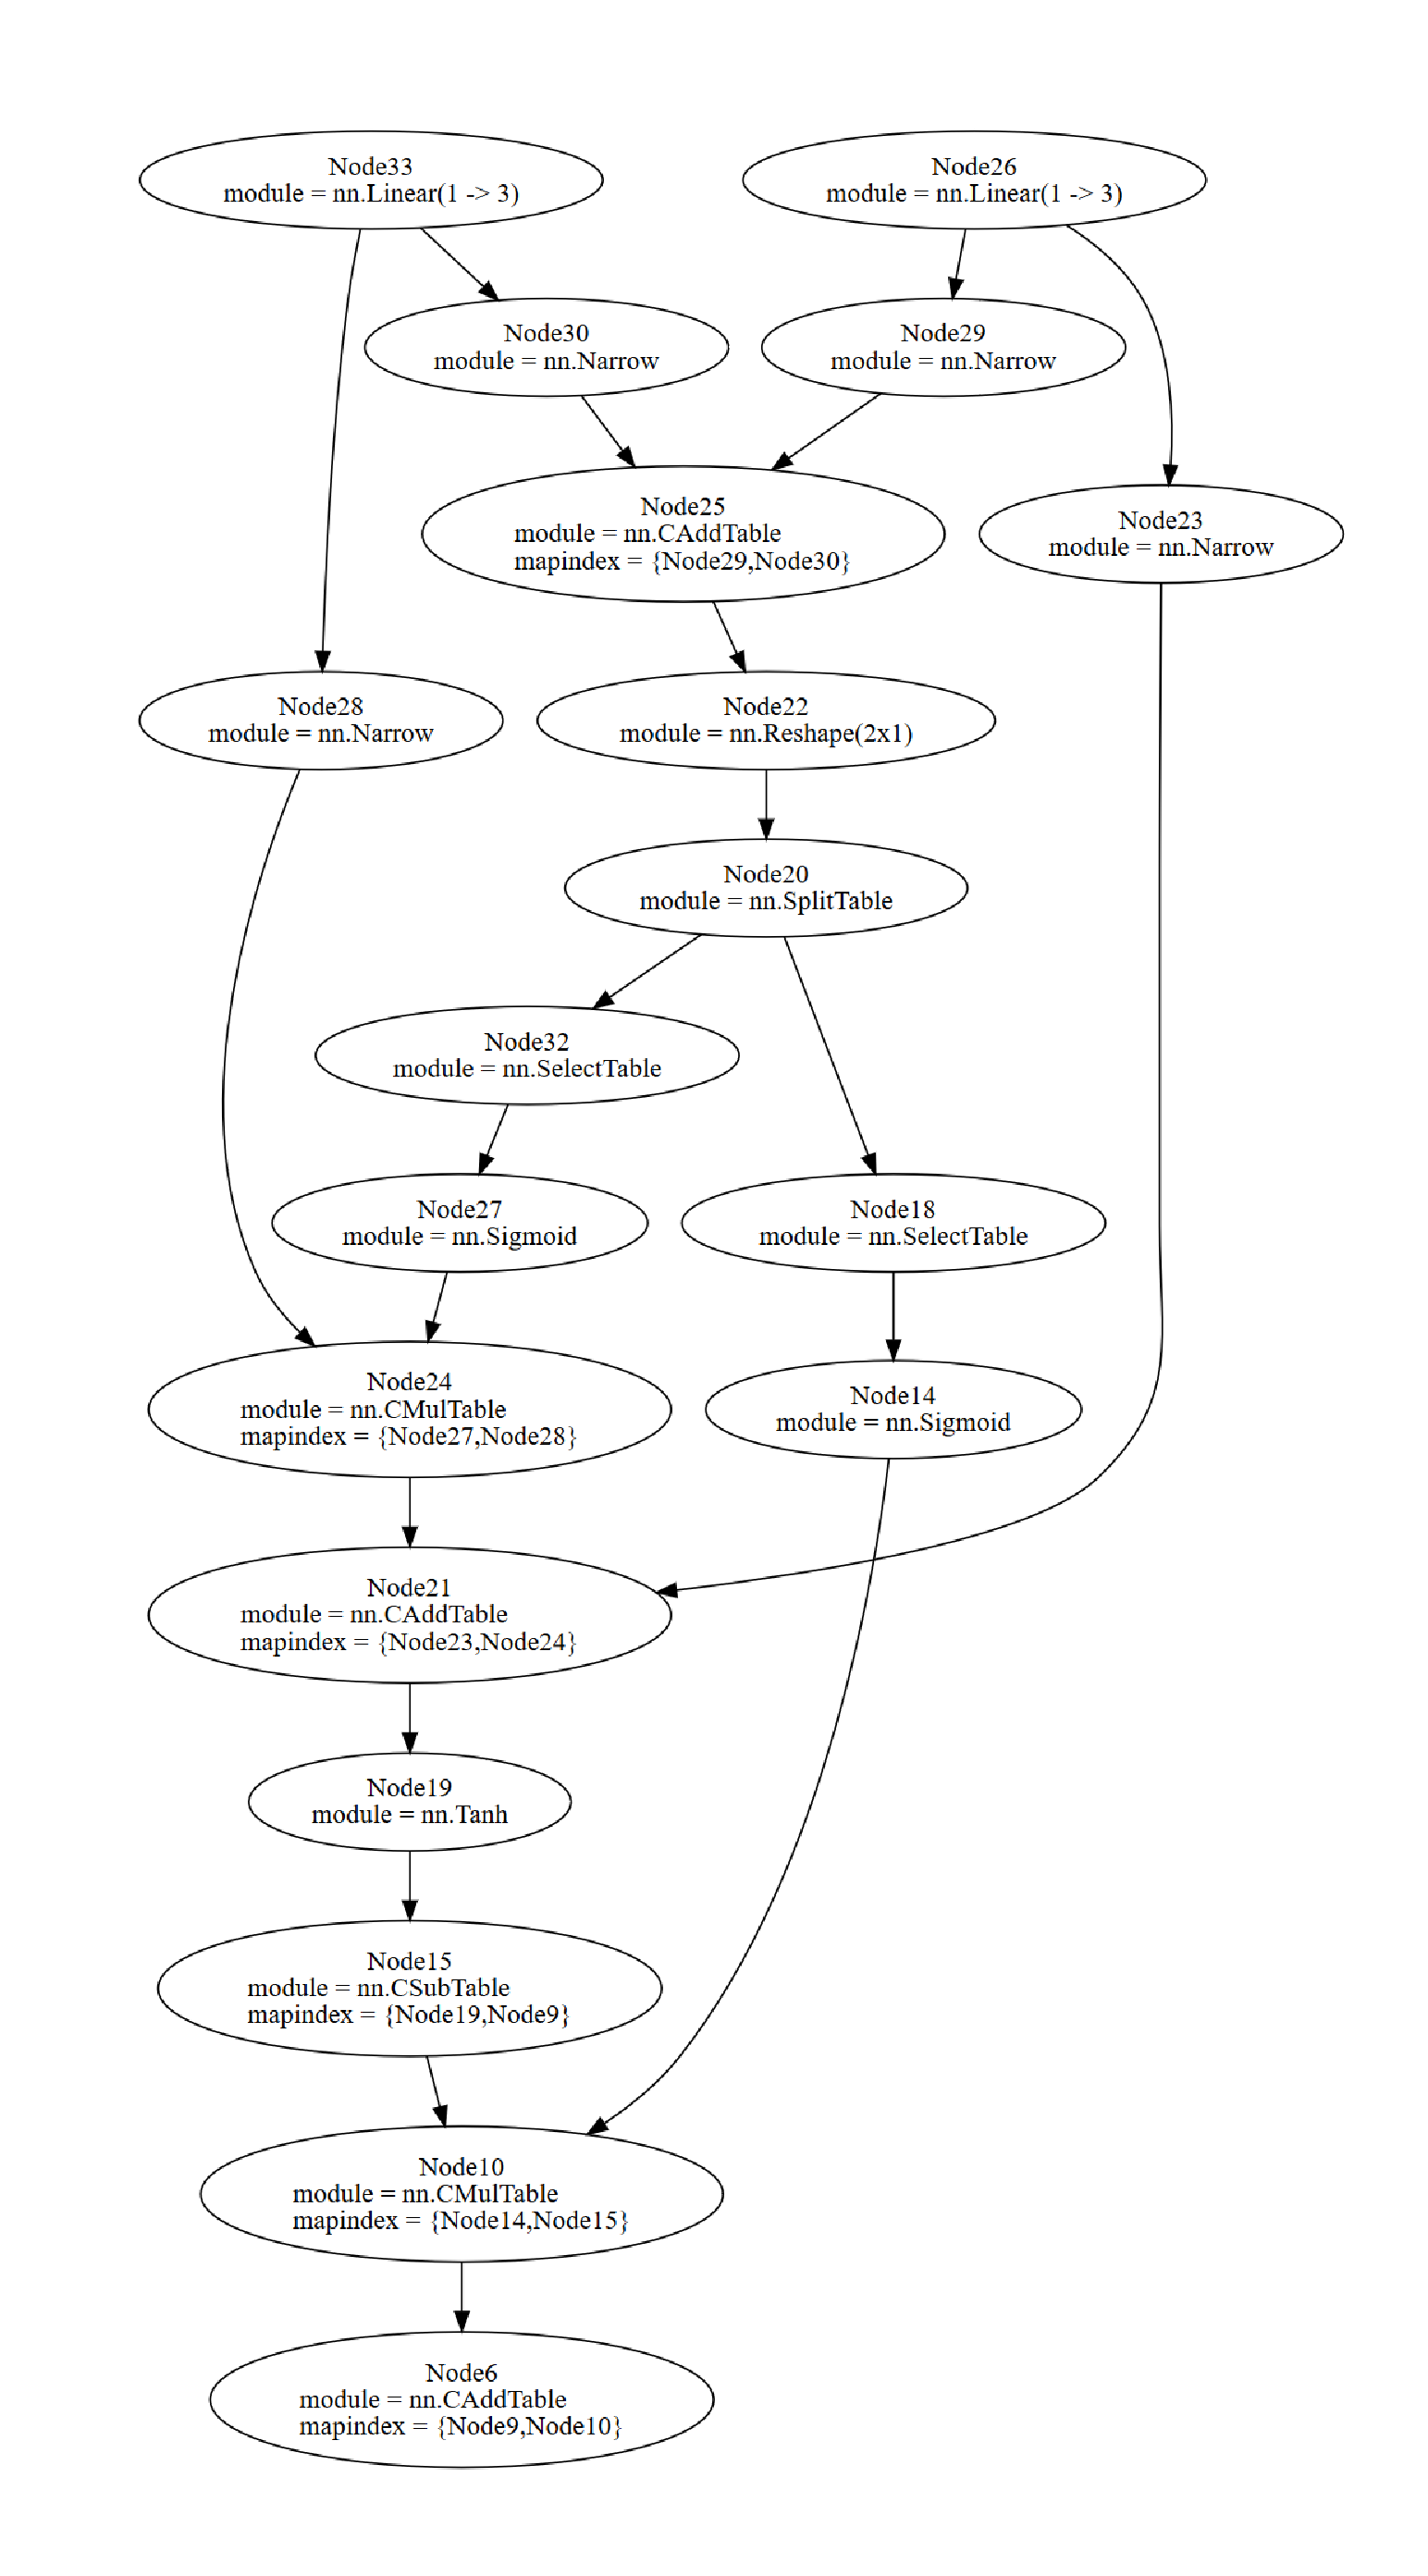
\includegraphics[height=1\textheight]{true}
  \caption{GRUCell given in slide 32 of talk by Armand Joulin\label{fig:gru_cell}}
\end{figure}

\section{Language Modeling}
\subsection{Generating sequences}
The query\_sentences.lua can be found at \url{https://git.io/vwQEc}.

The query\_sentences.lua does the following
\begin{enumerate}
  \item Loads the core network of the model.
  \item Builds the vocabulary map (max 10,000) and the inverse vocabulary map.
  \item Fetches the number of words to generate and the initial seed words (minimum 2).
  \item Does a forward pass on the core\_network for each and every word to generate the index for next word.
  \item The index is generated by using a multinomial distribution over the probabilities generated by the logsoftmax layer (layer 44 in core\_network)
  \item Concatenates and returns the new sentence.
\end{enumerate}

Steps to run the model:  \textit{th query\_sentences.lua}

\subsection{Improvements to the model}

\end{document}
